\documentclass[border=3pt]{standalone}
% Preâmbulo compartilhado pelos diagramas TikZ da aula 8 de IHR (Métodos de Pesquisa)
\usepackage[T1]{fontenc}
\usepackage[utf8]{inputenc}
\usepackage{lmodern}
\usepackage{amsmath}
\usepackage{xcolor}
\usepackage{tikz}
\usetikzlibrary{arrows.meta,angles,quotes,decorations.pathmorphing,decorations.pathreplacing,calc,
                positioning,shapes.geometric,shapes.misc,backgrounds,fit,
                math}

% Paleta (mesma dos SVGs originais)
% Paleta da disciplina de IHR: acento azul (#1A6FB5), cor de destaque do tema.
% (o nome "dblue" é mantido para não alterar todos os diagramas)
\definecolor{dblue}{HTML}{1A6FB5}
\definecolor{dorange}{HTML}{B3541E}
\definecolor{dgreen}{HTML}{4A7C59}
\definecolor{dred}{HTML}{9C4B4B}
\definecolor{dcream}{HTML}{F4F1EA}
\definecolor{dshade}{HTML}{DDD7C9}

% Função gaussiana (não normalizada por padrão de escala visual)
\pgfmathdeclarefunction{gauss}{3}{%
  \pgfmathparse{1/(#3*sqrt(2*pi))*exp(-((#1-#2)^2)/(2*#3^2))}%
}

% Estilos comuns (prefixo d... para não colidir com chaves internas do pgf)
\tikzset{
  >={Stealth[length=2mm]},
  dguide/.style={gray!55, dashed, line width=0.4pt},
  daxis/.style={gray!60, line width=0.7pt, ->},
  dbody/.style={fill=black!3, draw=black!80, line width=1pt},
  dacc/.style={draw=dblue, line width=1pt},
  dlbl/.style={black!55, font=\small},
  dsub/.style={black!45, font=\footnotesize},
  dstate/.style={circle, draw=black!80, fill=dcream, line width=1pt,
                 minimum size=17mm, font=\large, inner sep=1pt},
  dobs/.style={circle, draw=black!80, fill=dshade, line width=1pt,
               minimum size=14mm, font=\large, inner sep=1pt},
  dbox/.style={rounded corners=2pt, draw=black!80, fill=dcream, line width=1pt,
               align=center, inner sep=6pt},
  dop/.style={circle, draw=black!80, fill=white, line width=1pt,
              minimum size=6mm, inner sep=0pt, font=\small},
  dtrans/.style={->, dblue, line width=1pt},
  dmeas/.style={->, dorange, line width=1pt},
  dcurve/.style={line width=1pt, dblue},
  dcurveb/.style={line width=1.4pt, dorange},
}

\begin{document}
\hyphenpenalty=10000 \exhyphenpenalty=10000 \tolerance=9999 \emergencystretch=3em
\newcommand{\pessm}[4]{% x, y, contorno, preenchimento
  \draw[#3, fill=#4, line width=1.1pt] (#1,#2+0.3) circle (0.19);
  \draw[#3, fill=#4, line width=1.1pt, rounded corners=3pt] (#1-0.33,#2-0.42) rectangle (#1+0.33,#2+0.05);}
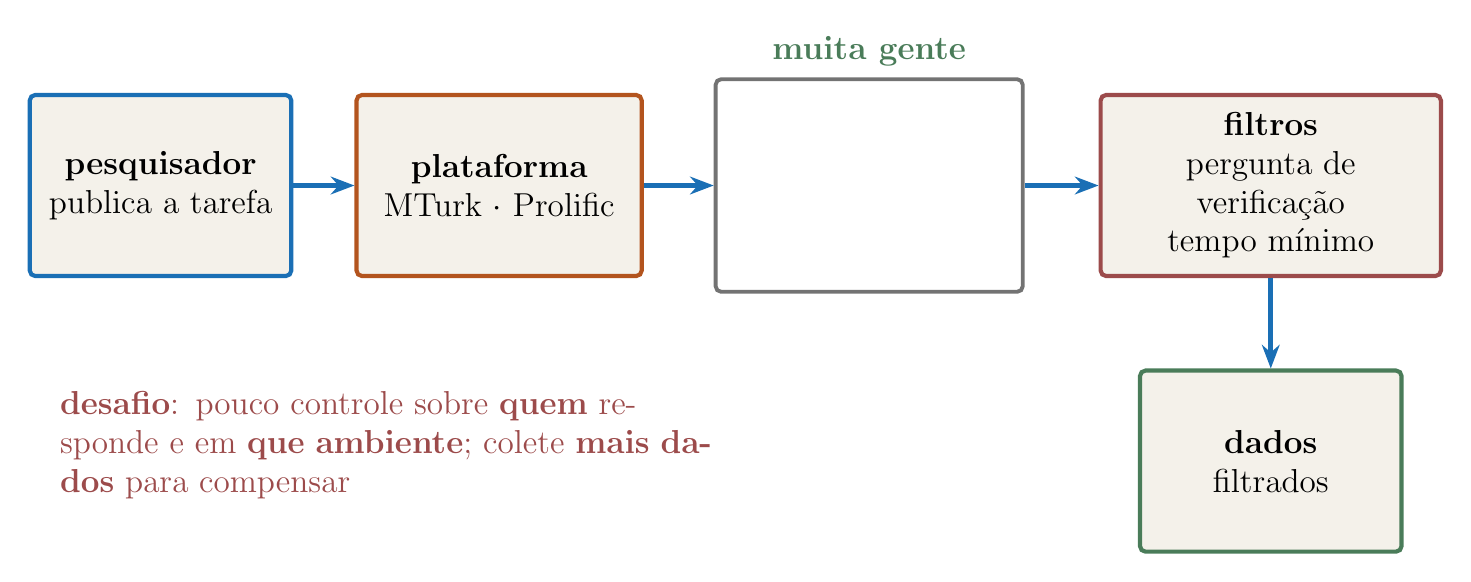
\begin{tikzpicture}[x=1cm,y=1cm]
  \tikzset{b/.style={dbox, minimum height=2.3cm, font=\large, line width=1.5pt, align=center}}
  \node[b, draw=dblue, text width=2.9cm] (p) at (1.7,4.4) {\textbf{pesquisador}\\ publica a tarefa};
  \node[b, draw=dorange, text width=3.2cm] (m) at (6.0,4.4) {\textbf{plataforma}\\ MTurk $\cdot$ Prolific};
  \node[dbox, draw=black!55, fill=white, line width=1.4pt, minimum width=3.9cm, minimum height=2.7cm] (g) at (10.7,4.4) {};
  \foreach \x in {9.4,10.2,11.0,11.8} {\foreach \y in {5.15,4.35,3.55} {\pessm{\x}{\y}{dgreen}{dgreen!12}}}
  \node[font=\large\bfseries, dgreen] at (10.7,6.1) {muita gente};
  \node[b, draw=dred, text width=3.9cm] (f) at (15.8,4.4) {\textbf{filtros}\\ pergunta de verificação\\ tempo mínimo};
  \node[b, draw=dgreen, text width=2.9cm] (d) at (15.8,0.9) {\textbf{dados}\\ filtrados};
  \draw[dtrans, line width=1.8pt, -{Stealth[length=3mm]}] (p.east) -- (m.west);
  \draw[dtrans, line width=1.8pt, -{Stealth[length=3mm]}] (m.east) -- (g.west);
  \draw[dtrans, line width=1.8pt, -{Stealth[length=3mm]}] (g.east) -- (f.west);
  \draw[dtrans, line width=1.8pt, -{Stealth[length=3mm]}] (f.south) -- (d.north);
  \node[font=\large, dred, text width=8.4cm, align=left, anchor=west] at (0.3,1.1) {\textbf{desafio}: pouco controle sobre \textbf{quem} responde e em \textbf{que ambiente}; colete \textbf{mais dados} para compensar};
\end{tikzpicture}
\end{document}
